\documentclass[twoside,11pt]{article}

% +
%  Name:
%     sun231.tex

%  Purpose:
%     SUN documentation for SCUBA ORAC-DR (SUN/231)

%  Authors:
%     Tim Jenness (JACH)

%  Copyright:
%     Copyright (C) 1997-2000 Particle Physics and Astronomy
%     Research Council. All Rights Reserved.
%
%  History:
%     $Log$
%     Revision 1.9  2004/05/27 20:11:18  bradc
%     udates for ORAC-DR v4.1-0
%
%     Revision 1.8  2004/01/09 23:51:24  bradc
%     describe correct looping behaviour at JCMT (-loop flag instead of -loop wait)
%
%     Revision 1.7  2001/04/12 00:03:52  timj
%     - v233.3
%     - add stardoccopyright
%     - add -file
%
%     Revision 1.6  2000/10/10 00:16:56  timj
%     Add fluxes to dependency list
%
%     Revision 1.5  2000/08/08 02:26:39  timj
%     Add csofit option.
%
%     Revision 1.4  2000/02/09 20:18:14  timj
%     Correct stardocnumber to .1 rather than .0
%
%     Revision 1.3  2000/02/08 04:41:11  timj
%     Fixes to documentation required by Starlink for release of V1.0-0
%
%     Revision 1.2  2000/02/03 09:50:33  timj
%     Add crossref to sun230
%
%     Revision 1.1.1.1  2000/02/03 09:44:58  timj
%     first starlink docs
%

%  Revision:
%     $Id$

% -

% ? Specify used packages
\usepackage{graphicx}        %  Use this one for final production.
\usepackage{times}
% \usepackage[draft]{graphicx} %  Use this one for drafting.
% ? End of specify used packages

\pagestyle{myheadings}

% -----------------------------------------------------------------------------
% ? Document identification
% Fixed part
\newcommand{\stardoccategory}  {Starlink User Note}
\newcommand{\stardocinitials}  {SUN}
\newcommand{\stardocsource}    {sun\stardocnumber}

% Variable part - replace [xxx] as appropriate.
\newcommand{\stardocnumber}    {231.4}
\newcommand{\stardocauthors}   {Tim Jenness, Frossie Economou\\
Joint Astronomy Centre, Hilo, Hawaii}
\newcommand{\stardocdate}      {June 2004}
\newcommand{\stardoccopyright} {Copyright \copyright\ 2004 Particle Physics and Astronomy Research Council}
\newcommand{\stardoctitle}     {ORAC-DR -- SCUBA Pipeline Data Reduction}
\newcommand{\stardocversion}   {4.1-0}
\newcommand{\stardocmanual}    {User's Manual}
\newcommand{\stardocabstract}  {%
\textsc{orac-dr} is a flexible data reduction pipeline designed to reduce
data from many different instruments. This document describes how
to use the \textsc{orac-dr} pipeline to reduce data taken with the
Submillimetre Common-User Bolometer Array (SCUBA) obtained from the
James Clerk Maxwell Telescope.
}
% ? End of document identification
% -----------------------------------------------------------------------------

% +
%  Name:
%     sun.tex
%
%  Purpose:
%     Template for Starlink User Note (SUN) documents.
%     Refer to SUN/199
%
%  Authors:
%     AJC: A.J.Chipperfield (Starlink, RAL)
%     BLY: M.J.Bly (Starlink, RAL)
%     PWD: Peter W. Draper (Starlink, Durham University)
%
%  History:
%     17-JAN-1996 (AJC):
%        Original with hypertext macros, based on MDL plain originals.
%     16-JUN-1997 (BLY):
%        Adapted for LaTeX2e.
%        Added picture commands.
%     13-AUG-1998 (PWD):
%        Converted for use with LaTeX2HTML version 98.2 and
%        Star2HTML version 1.3.
%     {Add further history here}
%
% -

\newcommand{\stardocname}{\stardocinitials /\stardocnumber}
\markboth{\stardocname}{\stardocname}
\setlength{\textwidth}{160mm}
\setlength{\textheight}{230mm}
\setlength{\topmargin}{-2mm}
\setlength{\oddsidemargin}{0mm}
\setlength{\evensidemargin}{0mm}
\setlength{\parindent}{0mm}
\setlength{\parskip}{\medskipamount}
\setlength{\unitlength}{1mm}

% -----------------------------------------------------------------------------
%  Hypertext definitions.
%  ======================
%  These are used by the LaTeX2HTML translator in conjunction with star2html.

%  Comment.sty: version 2.0, 19 June 1992
%  Selectively in/exclude pieces of text.
%
%  Author
%    Victor Eijkhout                                      <eijkhout@cs.utk.edu>
%    Department of Computer Science
%    University Tennessee at Knoxville
%    104 Ayres Hall
%    Knoxville, TN 37996
%    USA

%  Do not remove the %begin{latexonly} and %end{latexonly} lines (used by
%  LaTeX2HTML to signify text it shouldn't process).
%begin{latexonly}
\makeatletter
\def\makeinnocent#1{\catcode`#1=12 }
\def\csarg#1#2{\expandafter#1\csname#2\endcsname}

\def\ThrowAwayComment#1{\begingroup
    \def\CurrentComment{#1}%
    \let\do\makeinnocent \dospecials
    \makeinnocent\^^L% and whatever other special cases
    \endlinechar`\^^M \catcode`\^^M=12 \xComment}
{\catcode`\^^M=12 \endlinechar=-1 %
 \gdef\xComment#1^^M{\def\test{#1}
      \csarg\ifx{PlainEnd\CurrentComment Test}\test
          \let\html@next\endgroup
      \else \csarg\ifx{LaLaEnd\CurrentComment Test}\test
            \edef\html@next{\endgroup\noexpand\end{\CurrentComment}}
      \else \let\html@next\xComment
      \fi \fi \html@next}
}
\makeatother

\def\includecomment
 #1{\expandafter\def\csname#1\endcsname{}%
    \expandafter\def\csname end#1\endcsname{}}
\def\excludecomment
 #1{\expandafter\def\csname#1\endcsname{\ThrowAwayComment{#1}}%
    {\escapechar=-1\relax
     \csarg\xdef{PlainEnd#1Test}{\string\\end#1}%
     \csarg\xdef{LaLaEnd#1Test}{\string\\end\string\{#1\string\}}%
    }}

%  Define environments that ignore their contents.
\excludecomment{comment}
\excludecomment{rawhtml}
\excludecomment{htmlonly}

%  Hypertext commands etc. This is a condensed version of the html.sty
%  file supplied with LaTeX2HTML by: Nikos Drakos <nikos@cbl.leeds.ac.uk> &
%  Jelle van Zeijl <jvzeijl@isou17.estec.esa.nl>. The LaTeX2HTML documentation
%  should be consulted about all commands (and the environments defined above)
%  except \xref and \xlabel which are Starlink specific.

\newcommand{\htmladdnormallinkfoot}[2]{#1\footnote{#2}}
\newcommand{\htmladdnormallink}[2]{#1}
\newcommand{\htmladdimg}[1]{}
\newcommand{\hyperref}[4]{#2\ref{#4}#3}
\newcommand{\htmlref}[2]{#1}
\newcommand{\htmlimage}[1]{}
\newcommand{\htmladdtonavigation}[1]{}

\newenvironment{latexonly}{}{}
\newcommand{\latex}[1]{#1}
\newcommand{\html}[1]{}
\newcommand{\latexhtml}[2]{#1}
\newcommand{\HTMLcode}[2][]{}

%  Starlink cross-references and labels.
\newcommand{\xref}[3]{#1}
\newcommand{\xlabel}[1]{}

%  LaTeX2HTML symbol.
\newcommand{\latextohtml}{\LaTeX2\texttt{HTML}}

%  Define command to re-centre underscore for Latex and leave as normal
%  for HTML (severe problems with \_ in tabbing environments and \_\_
%  generally otherwise).
\renewcommand{\_}{\texttt{\symbol{95}}}

% -----------------------------------------------------------------------------
%  Debugging.
%  =========
%  Remove % on the following to debug links in the HTML version using Latex.

% \newcommand{\hotlink}[2]{\fbox{\begin{tabular}[t]{@{}c@{}}#1\\\hline{\footnotesize #2}\end{tabular}}}
% \renewcommand{\htmladdnormallinkfoot}[2]{\hotlink{#1}{#2}}
% \renewcommand{\htmladdnormallink}[2]{\hotlink{#1}{#2}}
% \renewcommand{\hyperref}[4]{\hotlink{#1}{\S\ref{#4}}}
% \renewcommand{\htmlref}[2]{\hotlink{#1}{\S\ref{#2}}}
% \renewcommand{\xref}[3]{\hotlink{#1}{#2 -- #3}}
%end{latexonly}
% -----------------------------------------------------------------------------
% ? Document specific \newcommand or \newenvironment commands.

% New commands
\newcommand{\oracdr}{\xref{\textsc{orac-dr}}{sun230}{}}
\newcommand{\oracsun}{\xref{SUN/230}{sun230}{}}

\newcommand{\task}[1]{{\textsf{#1}}}
\newcommand{\recipe}[1]{{\small\textsf{#1}}}
\newcommand{\primitive}[1]{{\small\texttt{#1}}}

\newcommand{\Kappa}{\xref{{\sc{Kappa}}}{sun95}{}}
\newcommand{\Fluxes}{\xref{{\sc{Fluxes}}}{sun213}{}}
\newcommand{\SURF}{\xref{{\sc{Surf}}}{sun216}{}}
\newcommand{\gaia}{\xref{{\sc{Gaia}}}{sun214}{}}
\newcommand{\cgsdr}{\xref{{\sc{cgs4dr}}}{sun27}{}}


\newcommand{\fitsmod}{\xref{\task{fitsmod}}{sun95}{FITSMOD}}
\newcommand{\qdraw}{\xref{\task{qdraw}}{sun216}{QDRAW}}
\newcommand{\extinction}{\xref{\task{extinction}}{sun216}{EXTINCTION}}
\newcommand{\scusetenv}{\xref{\task{scusetenv}}{sun216}{SCUSETENV}}


% Environment for indenting.
\newenvironment{myquote}{\begin{quote}\begin{small}}{\end{small}\end{quote}}


% ? End of document specific commands
% -----------------------------------------------------------------------------
%  Title Page.
%  ===========
\renewcommand{\thepage}{\roman{page}}
\begin{document}
\thispagestyle{empty}

%  Latex document header.
%  ======================
\begin{latexonly}
   CCLRC / \textsc{Rutherford Appleton Laboratory} \hfill \textbf{\stardocname}\\
   {\large Particle Physics \& Astronomy Research Council}\\
   {\large Starlink Project\\}
   {\large \stardoccategory\ \stardocnumber}
   \begin{flushright}
   \stardocauthors\\
   \stardocdate
   \end{flushright}
   \vspace{-4mm}
   \rule{\textwidth}{0.5mm}
   \vspace{5mm}
   \begin{center}
   {\Huge\textbf{\stardoctitle \\ [2.5ex]}}
   {\LARGE\textbf{\stardocversion \\ [4ex]}}
   {\Huge\textbf{\stardocmanual}}
   \end{center}
   \vspace{5mm}

% ? Add picture here if required for the LaTeX version.
%   e.g. \includegraphics[scale=0.3]{filename.ps}
\begin{center}

\includegraphics[width=1.0in]{sun231_sculogo.eps}
\hskip 1.0in

\includegraphics[width=1.0in]{sun231_logo.eps}
\end{center}
% ? End of picture

% ? Heading for abstract if used.
   \vspace{10mm}
   \begin{center}
      {\Large\textbf{Abstract}}
   \end{center}
% ? End of heading for abstract.
\end{latexonly}

%  HTML documentation header.
%  ==========================
\begin{htmlonly}
   \xlabel{}
   \begin{rawhtml} <H1> \end{rawhtml}
      \stardoctitle\\
      \stardocversion\\
      \stardocmanual
   \begin{rawhtml} </H1> <HR> \end{rawhtml}

% ? Add picture here if required for the hypertext version.
%   e.g. \includegraphics[scale=0.7]{filename.ps}

\includegraphics[width=1.0in]{sun231_sculogo.eps}

\includegraphics[width=1.0in]{sun231_logo.eps}
% ? End of picture

   \begin{rawhtml} <P> <I> \end{rawhtml}
   \stardoccategory\ \stardocnumber \\
   \stardocauthors \\
   \stardocdate
   \begin{rawhtml} </I> </P> <H3> \end{rawhtml}
      \htmladdnormallink{CCLRC / Rutherford Appleton Laboratory}
                        {http://www.cclrc.ac.uk} \\
      \htmladdnormallink{Particle Physics \& Astronomy Research Council}
                        {http://www.pparc.ac.uk} \\
   \begin{rawhtml} </H3> <H2> \end{rawhtml}
      \htmladdnormallink{Starlink Project}{http://www.starlink.rl.ac.uk/}
   \begin{rawhtml} </H2> \end{rawhtml}
   \htmladdnormallink{\htmladdimg{source.gif} Retrieve hardcopy}
      {http://www.starlink.rl.ac.uk/cgi-bin/hcserver?\stardocsource}\\

%  HTML document table of contents.
%  ================================
%  Add table of contents header and a navigation button to return to this
%  point in the document (this should always go before the abstract \section).
  \label{stardoccontents}
  \begin{rawhtml}
    <HR>
    <H2>Contents</H2>
  \end{rawhtml}
  \htmladdtonavigation{\htmlref{\htmladdimg{contents_motif.gif}}
        {stardoccontents}}

% ? New section for abstract if used.
  \section{\xlabel{abstract}Abstract}
% ? End of new section for abstract
\end{htmlonly}

% -----------------------------------------------------------------------------
% ? Document Abstract. (if used)
%  ==================
\stardocabstract
% ? End of document abstract

% -----------------------------------------------------------------------------
% ? LateX Copyright Statement
%  =========================
\begin{latexonly}
\newpage
\vspace*{\fill}
\stardoccopyright
\end{latexonly}
% ? End of Latex copyright statement

% -----------------------------------------------------------------------------
% ? Latex document Table of Contents (if used).
%  ===========================================
  \newpage
  \begin{latexonly}
    \setlength{\parskip}{0mm}
    \tableofcontents
    \setlength{\parskip}{\medskipamount}
    \markboth{\stardocname}{\stardocname}
  \end{latexonly}
% ? End of Latex document table of contents
% -----------------------------------------------------------------------------
\cleardoublepage
\renewcommand{\thepage}{\arabic{page}}
\setcounter{page}{1}


\section{Introduction\xlabel{introduction}}

The ORAC Data Reduction pipeline (\oracdr) is a general purpose pipeline for
reducing data from any instrument. A set of data reduction recipes are
available for use with reducing data from the Submillimetre Common-User
Bolometer Array (SCUBA) \cite{mnscu} at the \htmladdnormallinkfoot{James Clerk
Maxwell Telescope}{http://www.jach.hawaii.edu/JACpublic/JCMT/}, Mauna Kea,
Hawaii .  This document explains how to run the \oracdr\ data reduction
pipeline system on data taken with SCUBA.

Information on the general aspects of \oracdr\ (with more information on loop
control and the display system) can be found in document \oracsun.




\section{Pipeline Setup\xlabel{pipeline_setup}}

In order to configure the \oracdr\ SCUBA data reduction pipeline a setup
command, \texttt{oracdr\_scuba}, is provided. Assuming you are running the
command from the Unix \texttt{TC-shell}\footnote{\oracdr\ requires
\texttt{tcsh} for full functionality from the system setup. If \texttt{tcsh}
is not available the startup scripts (\texttt{oracdr\_ufti} etc) will not set
the specified UT date (the argument is ignored). In this case the
\texttt{ORAC\_DATA\_IN} and \texttt{ORAC\_DATA\_OUT} environment variables
must be set up explicitly.  Additionally, the \texttt{oracdr} command must
include the `\textbf{-ut}' option as specified in the \texttt{oracdr}
documentation.} this command sets all the environment variables and command
aliases required to run the pipeline.  The UT date of the observations can be
specified by supplying an argument to the command, if not specified the
current UT date is assumed:

\begin{myquote}
\begin{verbatim}
% oracdr_scuba 19990703
\end{verbatim}
\end{myquote}

In order for the startup script to be configured to read the
input data, an environment variable must be set which points
to the directory containing the UT date directory. For example,
if your data is in directory \texttt{/mydata/19991012} the following
is required:

\begin{myquote}
\begin{verbatim}
% setenv ORAC_DATA_ROOT /mydata
% oracdr_scuba 19991012
\end{verbatim}
\end{myquote}

If \texttt{ORAC\_DATA\_ROOT} is not set then the current directory
will be assumed unless the script is run at the Joint Astronomy Centre.
With this variable unset when run at the Joint Astronomy Centre
the input data directory will be configured to point to the actual
SCUBA archive data directory.

When run, this command should list information detailing the
current setup. Hopefully, it should be obvious at this point
whether something has gone wrong. Here is an example for the JAC:

\begin{myquote}
\begin{verbatim}
% oracdr_scuba 20000127

     ORAC Data Reduction Pipeline -- (ORAC-DR Version 1.0-0)
     Configured for instrument SCUBA

     Type "oracdr -h" for usage
     Type 'showme sun231' to browse the hypertext documentation


 Raw data will be read from /scuba/m99b/20000127/
 Reduced data will appear in /users/timj/oracdr/docs/sun231

+++++++++ For online SCUBA reduction use oracdr -loop flag +++++++++

For comments specific to SCUBA data reduction mail timj@jach.hawaii.edu
For problems with the ORAC-DR system mail helpme@jach.hawaii.edu
         http://www.jach.hawaii.edu/UKIRT/software/oracdr/

\end{verbatim}
\end{myquote}

A warning is printed if the input directory can not be found
on the system.

Once this is done, the next step is to set the location of the
output directory. By default, the directory from which the
\texttt{oracdr\_scuba} command was issued is chosen. In order
to override this value, the \texttt{ORAC\_DATA\_OUT} environment
variable must be set:

\begin{myquote}
\begin{verbatim}
% setenv ORAC_DATA_OUT /largedisk/myoracata/
\end{verbatim}
\end{myquote}

All \oracdr\ output files will appear in \texttt{ORAC\_DATA\_OUT}.
For more information on the \oracdr\ environment variables please
see \xref{SUN/230}{sun230}{shell_variables}.

\section{Running \oracdr\xlabel{running_orac_dr}}

Once the environment has been configured the \texttt{oracdr} command
will be available. Help on the available command line options
can be listed by invoking \texttt{oracdr -h}. In its simplest
form with no options, the pipeline will launch a logging window and
start processing data from observation number 1 until no more data are
available. For example\footnote{On an xterm that supports ANSI colour (e.g.\
\texttt{dtterm}) the output from \oracdr\ is colour coded depending on the
source of the message}:

\begin{myquote}
\begin{verbatim}
% oracdr
Orac says: No UT date supplied, using 19981001
ORAC says: Starting up monoliths...Done
Setting up display infrastructure (display tools will not
be started until necessary)...Done
No observation numbers supplied - starting from obs 1
Checking for next data file: 19981001_dem_0001.sdf....
\end{verbatim}
\end{myquote}
Note that the default setting is that \oracdr\ will use the current UT
date and start looking for observation number 1 in the \texttt{ORAC\_DATA\_IN}
directory. It will wait for a flag file to appear until the timeout period expires
(1 hour) or until the pipeline is aborted with CTRL-C. This behaviour
is equivalent to running \oracdr\ with the following options:
\begin{myquote}
\begin{verbatim}
% oracdr -from 1 -loop flag
\end{verbatim}
\end{myquote}

In many cases this is the correct behaviour at the telescope. In order to
modify the behaviour of \oracdr\ command-line options can be used.

\subsection{Selecting a UT date\xlabel{selecting_a_ut_date}}

The UT date is required so that the names of the raw data files can be
derived via observation numbers. The \textbf{-ut} option can be used
to specify the UT date of interest. For example,

\begin{myquote}
\begin{verbatim}
% oracdr -ut 19980715
\end{verbatim}
\end{myquote}

Currently, the pipeline can only process data from a single UT date in any
single invocation.  Data from multiple nights can not be coadded (even if they
are in the same directory since the filename is derived from the
UT)\footnote{This can be overcome by using soft links to rename the input files
-- see TJ for more information}.

In general, the \texttt{oracdr\_scuba} can be used to configure the
UT date so that the \textbf{-ut} flag will not be required.
Rerun \texttt{oracdr\_scuba} when data from a different UT date are to
be reduced.

\subsection{Choosing the observations\xlabel{choosing_the_observations}}

In many cases only a subset of the data in \texttt{ORAC\_DATA\_IN} are to be
processed. \oracdr\ provides a number of ways of specifying observations
either as a range of observation numbers or as a list.

The options are:

\begin{description}
\item[-from] \mbox{}

Specify the number of the first observation to be processed.
This option defaults to `1' if this option is omitted but the \textbf{-to} is
present.

\item[-to] \mbox{}

Specify the number of the last observation to be processed. If
the \textbf{-from} option is present but no \textbf{-to} option, then
all the data will be processed starting from \textbf{-from}.

\item[-list] \mbox{}

Specify a list of observations. This list should be comma-separated. Colons
can be used to indicate a range. For example, \textbf{-list 1,2,3,5:10,15}
would process observations 1,2,3,5,6,7,8,9,10 and 15.

\item[-file] \mbox{}

Specify a file containing names of files to be processed. This is useful
for procesing data taken on different nights.

\end{description}

Here are some examples of selecting observations using \oracdr:

\begin{myquote}
\begin{verbatim}
% oracdr -from 5
\end{verbatim}
\end{myquote}
Start at observation 5 and continue incrementing the observation number
until no more files are available.
\begin{myquote}
\begin{verbatim}
% oracdr -from 5 -to 20
% oracdr -list 5:20
\end{verbatim}
\end{myquote}
Start at observation 5 and finish at observation 20.

\begin{myquote}
\begin{verbatim}
% oracdr -to 20
\end{verbatim}
\end{myquote}
Start at observation 1 and finish at observation 20.

\begin{myquote}
\begin{verbatim}
% oracdr -list 1,2,3,4,5,20:25,30:32
\end{verbatim}
\end{myquote}
Process observations 1,2,3,4,5,20,21,22,23,24,25,30,31 and 32.

\begin{myquote}
\begin{verbatim}
% oracdr -file myfile.dat
\end{verbatim}
\end{myquote}

Process observations lists in texttt{myfile.dat}.

\subsection{Looping schemes\xlabel{looping_schemes}}

There are a number of different ways of dealing with the data detection
loop in \oracdr. If the system is being used `off-line', the data are
all present in the input directory and the pipeline assumes that no new
data will appear. In this case the \textit{list} and \textit{inf} detection
loops are supplied which stop processing when data files can no longer
be found. These are the default loops whenever observation
numbers are specified with \textit{list} being used in conjunction with the
\textbf{-list} and \textbf{-from/-to} options and \textit{inf} being
used in conjunction with the \textbf{-from} option.

At the telescope new data are continually arriving so a different detection
loop is required. The \textit{wait} loop is used

Occasionally observation numbers are skipped (e.g.\ when an observation is
aborted and not copied to the Sun). In this case the \textbf{-skip} option
should be used. Without this option the data detection loop aborts when
an observation can not be found (or it continues to wait for a file even
though an observation with a higher number now exists).
It is probably a good idea to always use the \textbf{-skip}
option when processing SCUBA data.


\section{Calibration\label{sec:cal}\xlabel{calibration}}

The calibration system can be configured using the \textbf{-cal} option.
For SCUBA this option can be used to decide how to obtain the sky opacity,
which gains to use and which bolometers should be turned off.

Jiggle map and photometry observations are automatically calibrated
by the pipline (maps can be calibrated in Jy/beam or Jy/arcsec$^2$
by configuring the recipe).

The arguments to \textbf{-cal} should be comma-separated
keyword=value pairs. The recognised keywords are:

\begin{itemize}
\item \textbf{gains} \mbox{}

This keyword controls the way that gain values are determined. The options
are:

\begin{description}
\item[default:] Use generic values for the gain (e.g.\ use 240 Jy/V at 850
microns). This is the default option.
\item[index:] Derive gains by using the gains index file. The index file
is updated every time a calibration observation is reduced (e.g.\ photometry
on a planet). The nearest calibration (in
time) will be used for the gain determination. An error will occur if
no calibration observation has been taken (or reduced) before an observation
is reduced.
\end{description}


\item \textbf{tausys} \mbox{}

This keyword controls the behaviour of the tau correction. The options
are:

\begin{description}
\item[CSO:] Derive taus for all wavelengths by using the CSO tau stored in the
header of each frame. This only works if the CSO tau is being updated.
\item[skydip:] Derive taus by using the skydip index file. The index file
is updated every time a skydip observation is reduced. The nearest skydip (in
time) will be used for the extinction correction.
If no skydip observation has been taken (or reduced) before an observation
is reduced the CSO tau value will be used. Warnings are issued if the
selected skydip was taken more than 3 hours from the current
observation.
\textbf{index} is an allowed synonym for \textbf{skydip}.
\item[a number:] If a number is given it is assumed to be a CSO tau value.
A value of 0.0 will turn off extinction correction.
\item[850skydip:] Derive taus by using the 850 skydip values. Tau values
from other filters are all derived from the 850 value using the standard
tau ratios. If no suitable skydip can be found the CSO tau value will be
used. Warnings are issued if the
selected skydip was taken more than 3 hours from the current
observation.
\item[dipinterp \& 850dipinterp:] Same as \textbf{skydip} and
\textbf{850skydip} except values either side of the current observation
are interpolated to find the current tau. This is \emph{not} the same as
specifying two tau values to the \SURF\ \extinction\ task since that
will calculate the interpolated tau throughout the time of the observation
rather than just calculating the value for the start. If only one value can
be found then that value is used; if no values are found then CSO will
be used. Warnings are issued if skydips were taken more than 3 hours from
the current observation.
\item[csofit:] Derive the CSO tau (and hence the tau for the specified
filter) by using a polynomial fit to the CSO data for each night. This is the
most accurate method of determining the opacity but is only available
for nights between April 1997 and February 2001 (more fits will be provided
as they become available). This method has the added advantage that
photometrically unstable nights will not have a fit and therefore will
not be processed (useful when processing large numbers of observations
automatically).
\end{description}

\item \textbf{badbols} \mbox{}

This keyword controls the selection of bad bolometers (i.e.\ bolometers
turned off by the pipeline). The options are:

\begin{description}
\item[index:] Uses an index file containing bad bolometers. The index
file is written by the \recipe{SCUBA\_NOISE} recipe and contains a list
of all bolometers that had noise (from REFLECTOR observations) greater than
the specified threshold limit (currently the default threshold is 100\,nV).
\item[file:] Uses a file \verb|badbol.lis| found
in \texttt{ORAC\_DATA\_OUT}.
The file should contain a single line containing a space-separated list
of bolometer names\footnote{Bolometer numbers can not be used since that
depends on the sub-instrument in use}. The file may contain a line such as:
\begin{myquote}
\begin{verbatim}
A1 E2 H7 I5
\end{verbatim}
\end{myquote}
This is the default system.
\item[a list of bolometers:] Finally, it is possible to specify a list of
bolometer names. This list should be colon-separated, e.g.: `H7:A2:b3'

\end{description}

\end{itemize}

Here are some examples:

\begin{myquote}
\begin{verbatim}
% oracdr -cal tausys=skydip
\end{verbatim}
\end{myquote}
Derive opacities from the index file but use the default gains.
\begin{myquote}
\begin{verbatim}
% oracdr -cal gains=index,tausys=0.08
\end{verbatim}
\end{myquote}
Use a constant value for the opacity and use the derived gains
from the index file.
\begin{myquote}
\begin{verbatim}
% oracdr -cal tausys=850dipinterp
\end{verbatim}
\end{myquote}
Use the 850 micron skydips either side of an observation
to derive all taus. Use the standard gain values.
\begin{myquote}
\begin{verbatim}
% oracdr -cal badbols=a3:c14
\end{verbatim}
\end{myquote}
Turn off bolometers a3 and c14.


\section{Recipes\xlabel{recipes}}

Data reduction recipes exist for processing data from the standard SCUBA
observing modes. This does limit the flexibility of any given recipe since
they are designed to work for any data from that mode. Occasionally it is
necessary to modify recipes (e.g.\ change the sky bolometers or size of pixels to
be used for the rebinning) and this can be achieved in a number of ways:

\begin{enumerate}

\item Specify a new recipe name on the command line. This is fine
for reducing observations taken in the same way but should not be used
in the general case since this command line argument overrides all
recipe choices regardless of observation mode.

\item Create a recipe with a different name and store this name
in the header before the observation is taken. This is done by using
the \texttt{DRRECIPE} ODF parameter.

\item Create a recipe with a different name and modify the \texttt{DRRECIPE}
FITS header value using the \Kappa\ \fitsmod\ command.


\item Use the \texttt{ORAC\_RECIPE\_DIR} environment variable. This variable
should be set before running up \oracdr\ and provides a search path that is
used to locate recipes. When \oracdr\ attempts to read a recipe it first looks
in \texttt{ORAC\_RECIPE\_DIR}, then in \texttt{ORAC\_DIR/recipes/SCUBA} (the
default location) and finally in the current directory (which will be
\texttt{ORAC\_DATA\_OUT}).

In order to modify a recipe, it should be copied from the default location
(\texttt{ORAC\_DIR/recipes/SCUBA}) to \texttt{ORAC\_RECIPE\_DIR} and edited there. The next
time \oracdr\ tries to read the recipe the modified version will be used
in preference to the standard version.

\end{enumerate}

The standard SCUBA recipes are:

\begin{description}
\item[\recipe{SCUBA\_NOISE}] for noise observations
\item[\recipe{SCUBA\_STD\_PHOTOM}] for photometry observations
\item[\recipe{SCUBA\_JIGMAP}] for jiggle map reduction
\item[\recipe{SCUBA\_POINTING}] for array pointing observations
\item[\recipe{SCUBA\_EM2SCAN}] for SCAN/MAP data reduction using the Emerson II
technique \cite{EII}.
\item[\recipe{SCUBA\_SKYDIP}] for skydip observations.
\item[\recipe{SCUBA\_JIGPOLMAP}] for array polarimetry (jiggle maps)
\item[\recipe{SCUBA\_EKHSCAN}] for scan/map data reduction using the EKH \cite{ekh} technique
\end{description}

Null recipes are provided for ALIGN, and FOCUS observations.


\section{Bad bolometers\xlabel{bad_bolometers}}

In some cases data are affected by the presence of excessively noisy
bolometers. To overcome this problem a facility is provided for turning
off specific bolometers so that they are ignored by the data reduction.

See the section on calibration (\S\ref{sec:cal}) for more information on how
to set bolometers to bad using the \texttt{badbols} calibration option.


\section{Bad observations\xlabel{bad_observations}}

In some cases, it is desirable to remove some frames (observations)
from a group. For example, you make 5 observations of a source
but you see that when the pipeline combines observation 3 into the
group the noise is dominated by this observation. In order
not to contaminate the group when observations 4 and 5 are coadded
the pipeline must be instructed to remove observation 3 from any further
group operations.

Observations can be turned off by using a special type of
\oracdr\ index file (cf. index files generated by skydip and
calibration observations).

This index file is called \texttt{index.badobs} and should be present in the
\texttt{ORAC\_DATA\_OUT} directory. It should contain a line for each observation to be
removed. Each line should contain the observation number and the 8 digit UT
date (YYYYMMDD), e.g.:

\begin{quote}
\begin{verbatim}
55  19990128
62  19990129
\end{verbatim}
\end{quote}



\section{Bad integrations\xlabel{bad_observations}}

Currently it is not possible to turn off specific integrations
using the pipeline.

\section{Processing specific sub-instruments\xlabel{processing_specific_sub_instruments}}

By default all sub-instruments are processed by the pipeline. In some
cases, e.g.\ where there is no hope of detecting anything at 450 microns,
this is undesirable since this doubles the time required by the pipeline
to process each observation. To overcome this the recipe can be
edited to select specific sub-instruments as follows:

\begin{enumerate}
\item Copy the recipe you are interested in to \texttt{ORAC\_RECIPE\_DIR}
(create this directory and set the environment variable if necessary). For
example, for scan maps copy \recipe{SCUBA\_EM2SCAN} from
\texttt{ORAC\_DIR/recipes/SCUBA} to \texttt{ORAC\_RECIPE\_DIR}

\item Change the \texttt{\_EXTINCTION\_CORRECT\_} line to
`\texttt{\_EXTINCTION\_CORRECT\_ SUBS=long}' to only process the LONG
sub-instrument. The SUBS argument can take a comma-separated list (e.g.\
P2000,LONG to select 2mm and LONG).

\end{enumerate}

A modified recipe may look something like:

\begin{myquote}
\begin{verbatim}
_PRE_PROCESS_
_FLAT_FIELD_
_SET_BAD_PIXELS_
_DESPIKE_SCAN_
_EXTINCTION_CORRECT_ SUBS=long
_REMOVE_SCAN_BASELINE_
_REMOVE_SKY_NOISE_SCAN_
_REBIN_FRAME_ PIXEL_SIZE=3.0 REBIN_METHOD=GAUSSIAN
_REBIN_EM2_GROUP_ PIXEL_SIZE=1.0 REBIN_METHOD=GAUSSIAN
\end{verbatim}
\end{myquote}

\section{The \oracdr\ display system\xlabel{the_orac_display_system}}

\oracdr\ uses a fully configurable display system. By default the data
display is turned on but can be turned off by using the \textbf{-nodisplay}
option when starting \oracdr. For a more general introduction to the
display system see \xref{SUN/230}{sun230}{display_system}.

The default configuration is to use \Kappa\ graphics commands via the
\textsc{kapview} monolith, and uses a single
\xref{GWM}{sun219}{}/\xref{GKS}{sun83}{} window split into sections. For
mapping observations the individual reduced frames are displayed in the top
two quadrants and reduced groups displayed in the lower quadrants (only one
quadrant is used per sub-instrument). For skydips and photometry observations
the display is split into two horizontal regions.

\subsection{Display systems\xlabel{display_systems}}

The \oracdr\ display interface currently can use \Kappa\ and
\gaia\footnote{The \xref{\textsc{p4}}{sun27}{} display engine is also supported, but
its use is deprecated}. The \gaia\ interface can only support image display
whereas the \Kappa\ (\textsc{kapview}) interface can support imaging, graphs, scatter
plots and vector plots.

\subsection{Display types\xlabel{display_types}}

\oracdr\ can be configured to use the following display types:

\begin{description}
\item[IMAGE:] Display an 2-D image file. The X,Y and Z limits can be
specified or autoscaling can be used. Supported by \gaia, \textsc{kapview} and \textsc{p4}.
\item[GRAPH:] Display a 1-D data set as a line graph. Supported by
\textsc{kapview} and  \textsc{p4}
\item[SIGMA:] Display a data set as a scatter plot with a Y-range specified in
sigmas and horizontal dashed lines at a specific sigma range
(useful for photometry data - equivalent to the \SURF\ routine \qdraw) (\textsc{kapview} only)
\item[DATAMODEL:] Display a 1-D data set (as points) with a model (as a solid
line). Designed for displaying skydip results. (\textsc{kapview} only)
\item[HISTOGRAM:] Show a histogram of all data (\textsc{kapview} only)
\item[VECTOR:] Show vectors on top of an image (\textsc{kapview} only)
\end{description}

\subsection{Configuring the \oracdr\ display system\xlabel{configuring_the_oracdr_display_system}}

The display is configured via the \texttt{oracdisp} tool and the
\texttt{disp.dat} file found in \texttt{ORAC\_DATA\_OUT}. The \texttt{oracdisp}
tool provides a graphical front-end to the display system and
can be used to control where images are displayed, what type of display
is used and how the data should be displayed. \texttt{oracdisp}
runs independently of the pipeline, the only interaction between
the pipeline and \texttt{oracdisp} is via a configuration file.
Each time a primitive requests that a data file should be displayed
the pipeline compares the graphics ID generated by the frame itself (usually
the last suffix) with the list of suffixes stored in the display configuration
file. If they match, the configuration file is read (including information
such as where to display it, the type of device and the bounds) and the
corresponding display engine is instructed to display the data file
using the supplied option. If multiple matches are made, then multiple
display requests are processed. In this way a single display request
from a primitive can be used to display multiple images (e.g.\ load an image
into \gaia\ and display a slice using \Kappa).


\begin{figure}
\begin{center}
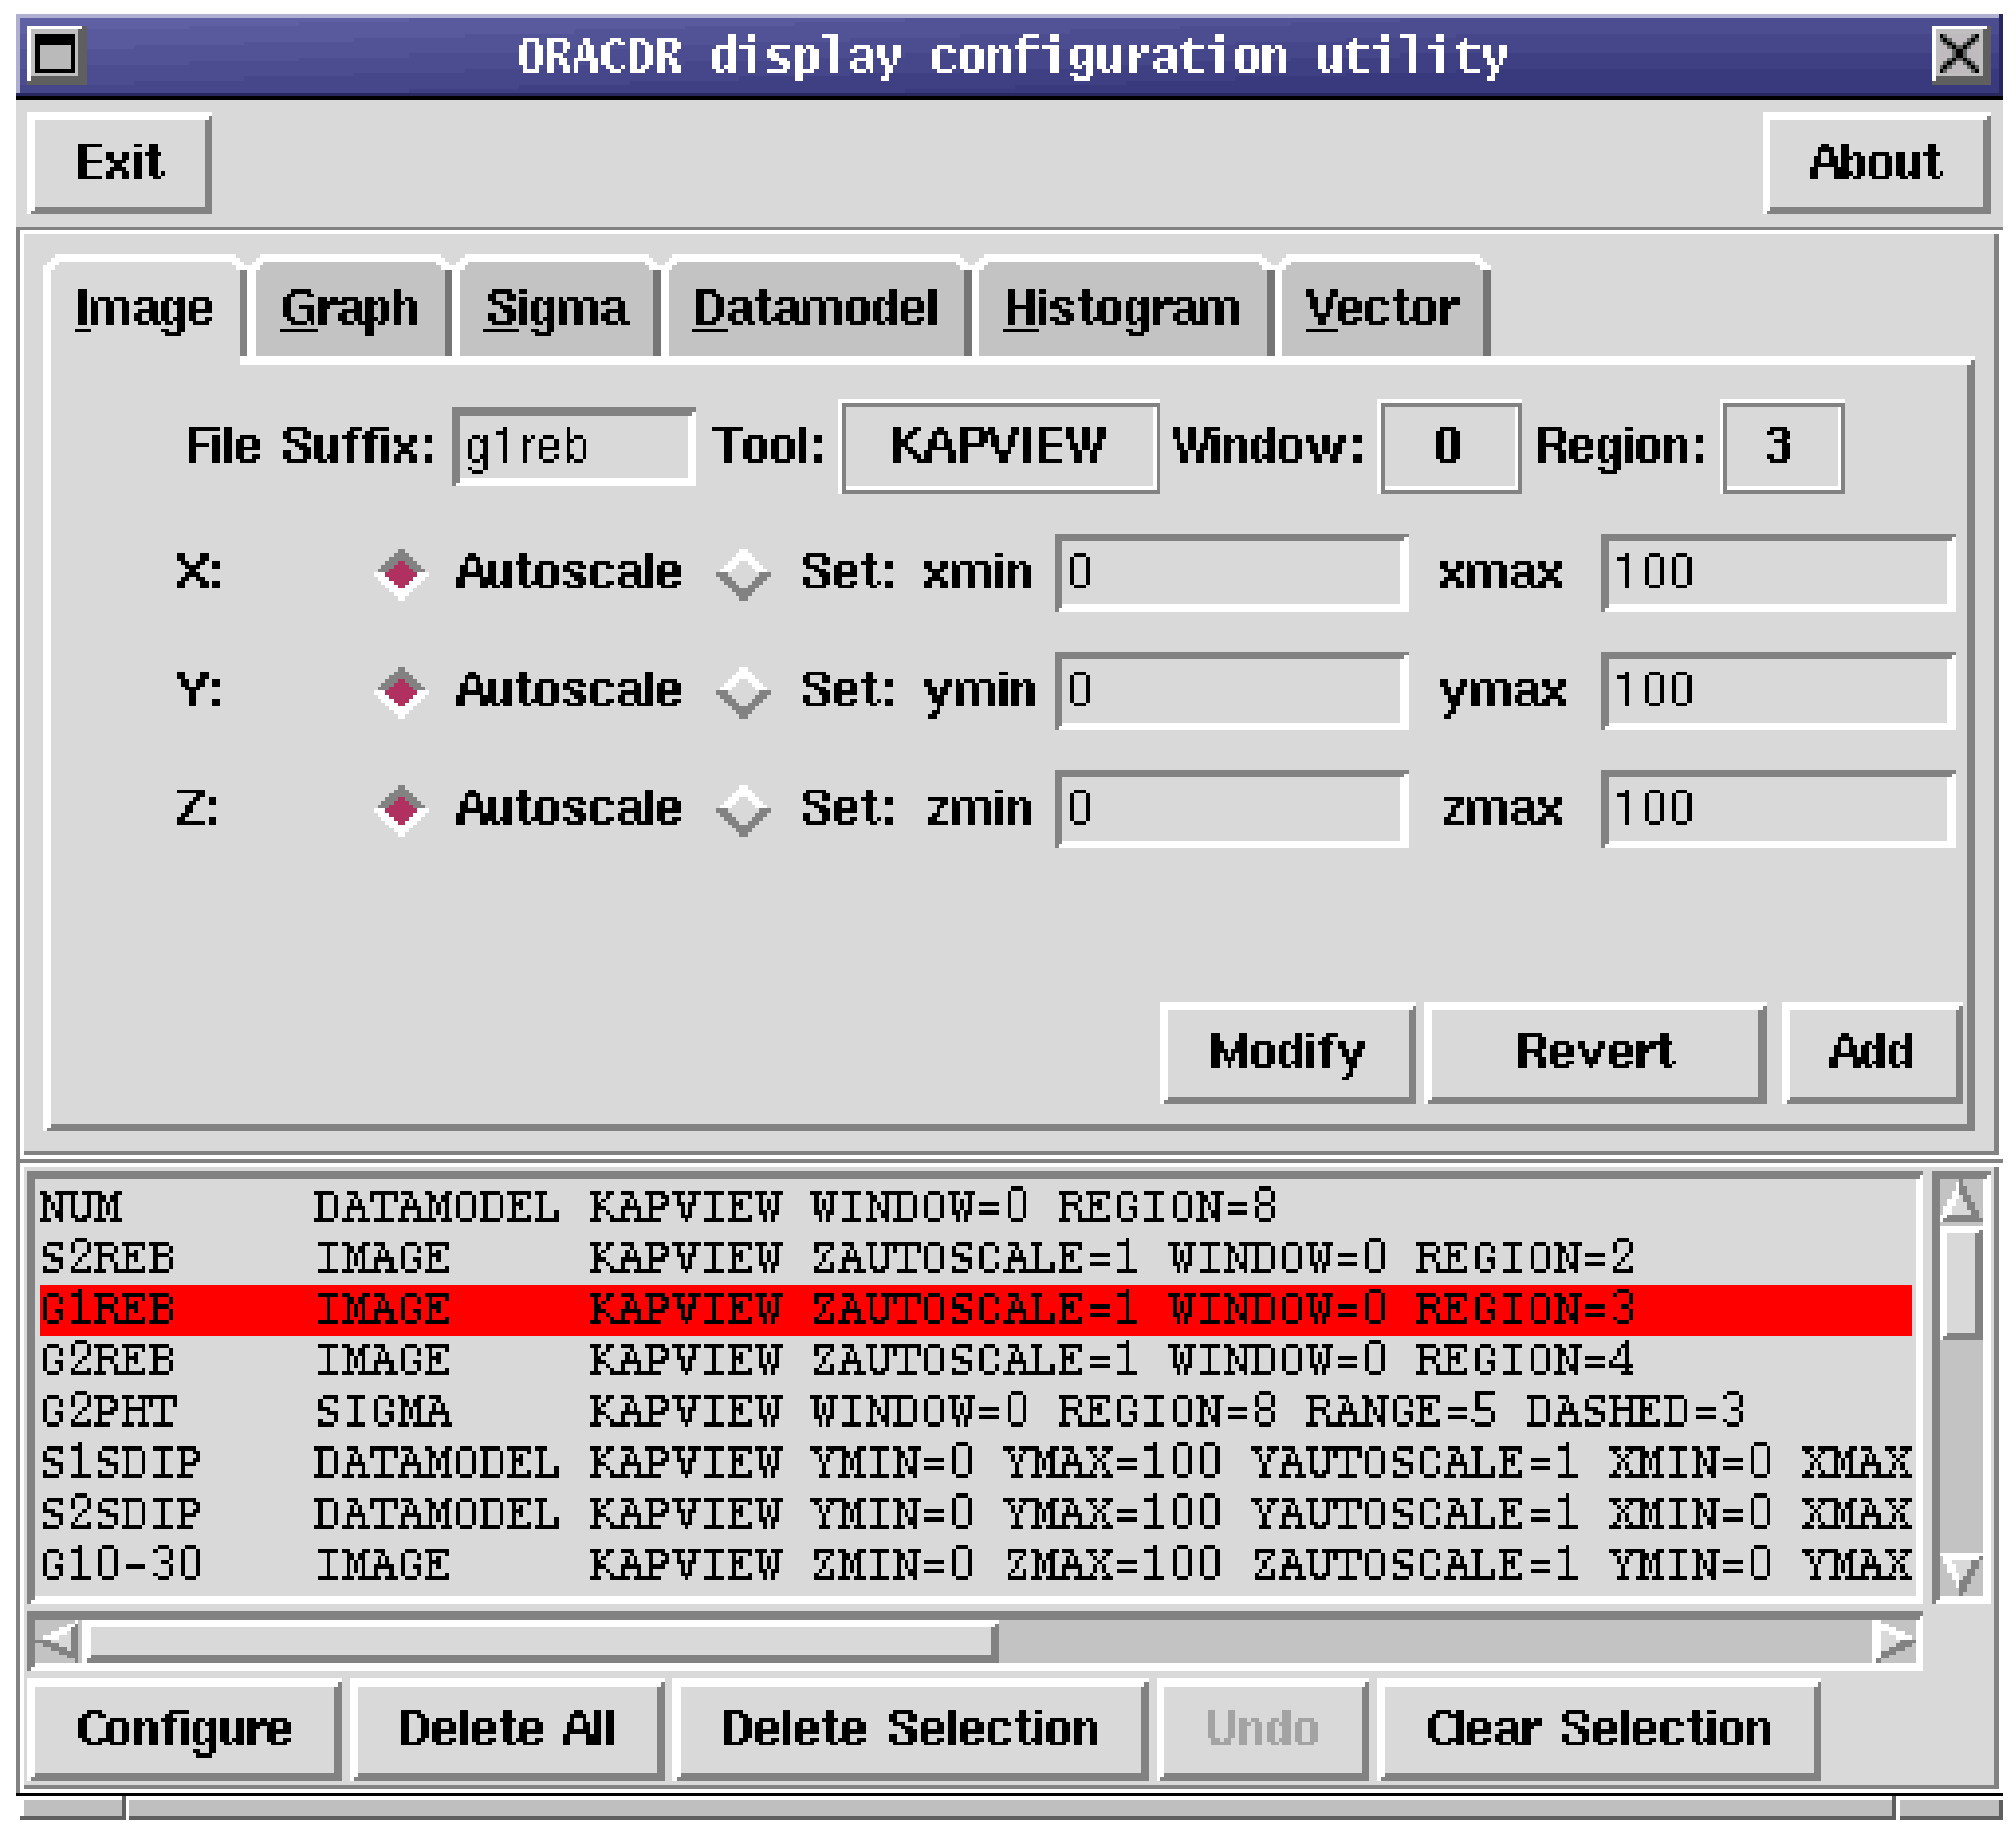
\includegraphics[width=\textwidth]{sun231_disp.eps}
\caption{The ORACDISP display configuration tool.}
\label{fig:oracdisp}
\end{center}
\end{figure}

The \texttt{oracdisp} tool is shown in figure \ref{fig:oracdisp}. The
tool is split into 3 major sections:

\begin{itemize}
\item A set of `pages' corresponding to each display type. This is where
the display details can be modified or details.
\item A lower window containing the current display
definition. Double-clicking on any line will select the entry and load the
information into the top frame. This can be used to copy an entry (e.g.\
by modifying the page details and pressing the `Add' button) or
modify the existing entry (pressing the `Modify' button will change the
highlighted entry - note that choosing a new page will reset the
selection). A single click on an entry will select it for deletion (see next item).

\item  The lower frame contains buttons for saving and modifying the
definition visible in the lower selection frame. The buttons do the following:
\begin{description}
\item[Configure:] This writes the current definition to disk (in
\texttt{ORAC\_DATA\_OUT/disp.dat}). No backup is made of the original file.
\item[DeleteAll:] Delete all entries in the selection frame
\item[DeleteSelection:] Delete all selected entries (entries are selected by a
single click - they are then highlighted in blue).
\item[Undo:] Undo a deletion
\item[ClearSelection:] Clear all selections.

\end{description}
\end{itemize}

The string that should be placed in the `File Suffix' entry
widget is discussed in the next section.

\subsection{Displaying frame output\xlabel{displaying_frame_output}}

For SCUBA data, the products of early stages of data reduction
(e.g.\ flatfielding or despiking) are not really suitable for display
so many of the early primitives do not contain display directives.

Table \ref{tab:framegui_id} lists the suffices along with the primitives that
generate the display request (and therefore must be called in the recipe).

\begin{table}
\begin{center}
\begin{tabular}{lll}
Suffix & Type of image &Primitives \\ \hline
noise&Noise & \_REDUCE\_NOISE\_  \\
sdip &Skydip & \_DISPLAY\_SKYDIP\_ \\
pht  &Photometrt data & \_DISPLAY\_PHOTOM\_GROUP\_ \\
reb  &Rebinned image & \_REBIN\_FRAME\_ \\
pol  &Polarisation (I,P,THETA) image & \_CALCULATE\_POLARISATION\_FRAME\_ \\
p    &Polarisation P image & \_CALCULATE\_POLARISATION\_FRAME\_ \\
theta&Polarisation THETA image& \_CALCULATE\_POLARISATION\_FRAME\_ \\
\hline
\end{tabular}
\caption{Suffix values used to display individual frames}
\label{tab:framegui_id}
\end{center}
\end{table}

Each of these suffixes can be prefixed by an `sN' prefix where `s' stands for
sub-instrument and N is a number indicating the position of the sub-instrument
in the raw data (for SCUBA N is usefully between 1 and 3). For example,
a display definition to display both the long and short rebinned images
should contain definitions identified by `s1reb' and `s2reb' whereas
`reb' would be relevant if only 1 sub-instrument is being processed.

\subsection{Displaying group output\xlabel{displaying_group_output}}


Table \ref{tab:groupgui_id} lists the group suffixes recognised by the
display system.
In a similar way to frame definitions, all group id's are prefixed
by `gN' where `g' indicates that a group is being displayed
and `N' is the sub-instrument number. Unlike for frames, the
gN prefix is always attached regardless of the number of sub-instruments
in the group.

The \primitive{\_REBIN\_EM2\_GROUP\_} primitive uses a gNpa-thr where `pa' refers
to the position angle of the chopped data and `thr' to the chop throw.
For example, to view the rebinned image of the data taken with
65 arcsec chop at 90 degrees position angle for the first sub-instrument
a display id of `g190-65' would be required.

\begin{table}
\begin{center}
\begin{tabular}{lll}
Suffix & Type of image &Primitives \\ \hline
gNreb  &Rebinned image & \_REBIN\_GROUP\_ \& \_REBIN\_EM2\_GROUP\_ \\
gNpa-thr & Rebinned dual-beam image & \_REBIN\_EM2\_GROUP\_ \\
gNpht & Photometry results & \_DISPLAY\_PHOTOM\_GROUP\_ \\
\hline
\end{tabular}
\caption{Suffix values used to display individual groups.}
\label{tab:groupgui_id}
\end{center}
\end{table}

\section{Release Notes}

\subsection{V1.0}

First release of ORAC-DR for SCUBA.

\subsection{V1.1}

\begin{itemize}
\item Add jiggle map calibration
\item Add support for wideband and narrow band filters
\end{itemize}

\begin{thebibliography}{}
\addcontentsline{toc}{section}{References}

\bibitem{mnscu}
Holland~W.~S., Robson~E.I., Gear~W.K., Lightfoot~J.~F., Jenness~T.,
Ivison~R.~J., Stevens~J.~A., Cunningham~C.~R., Ade~P.~A.~R.,
Griffin~M.~J., Duncan~W.~D., Murphy~J.~A., Naylor~D.~A., 1999,
\textit{MNRAS}, \textbf{303}, 659

\bibitem{EII}
Emerson~D.~T., Klein~U., Haslam~C.~G.~T., 1979, \textit{ApJ}, \textbf{76}, 92

\bibitem{ekh}
Emerson~D.~T., \textit{A.S.P. Conf. Ser} \textbf{75}, 309


\end{thebibliography}


\appendix

\section{Prerequisites\xlabel{prerequisites}}

The SCUBA \oracdr\ system requires the following Starlink packages
in addition to those packages required to simply run the
pipeline itself for a generic instrument:

\begin{itemize}
\item \SURF
\item \Kappa
\item \Fluxes
\end{itemize}

For polarimetry data reduction these additional packages are
required:

\begin{itemize}
\item \xref{\textsc{Polpack}}{sun223}{}
\item \xref{\textsc{Ccdpack}}{sun139}{}
\item \xref{\textsc{Cursa}}{sun190}{}
\end{itemize}


\section{Configuring the \oracdr\ environment\xlabel{configuring_the_orac_dr_environment}}

\oracdr\ uses environment variables to configure the global behaviour
of the data reduction pipeline. Environment variables specify the input
and output directories, the instrument type and the recipe/primitive
locations. In general these variables are set by the start up script.

The following variables are used by the pipeline:


\begin{description}
\item[\texttt{ORAC\_DIR}] \mbox{}

This is the location of the \oracdr\ software. At the JAC this will be
\verb|/jcmt_sw/oracdr|. This variable is set as part of the Starlink
login.

\item[\texttt{ORAC\_PERL5LIB}] \mbox{}

This is the location of the ORAC perl libraries. It should be set to
\verb|${ORAC_DIR}/lib/perl5|   %$
This variable is set as part of the Starlink login.

\item[\texttt{ORAC\_INSTRUMENT}] \mbox{}

This environment variable is used to inform \oracdr\ of the instrument
that is to be used by the pipeline. This configures the primitive and recipe
directories, file-naming conventions and other instrument specific
options. In order to process SCUBA data this environment variable should
be set to `SCUBA'. This is set by the \texttt{oracdr\_scuba} command.

\item[\texttt{ORAC\_DATA\_CAL}] \mbox{}

This variable should point to the directory containing the calibration
information. In SCUBA's case these are the files that determine the rules
that should be used for choosing skydip taus or gains.
This is set by the \texttt{oracdr\_scuba} command.
At JAC this should be set to \verb|/jcmt_sw/oracdr_cal/|.

\item[\texttt{ORAC\_DATA\_IN}] \mbox{}

This is the directory containing the raw data files. It is equivalent
to the \texttt{DATADIR} environment variable used by the \SURF\ software.
Currently \oracdr\ must use raw data -- partially processed data can not
be pipelined. At the telescope this is usually set to
\verb|/jcmtarchive/YYYYMMDD/|. The \SURF\ command \scusetenv\
can be used to set this variable automatically (with no argument
the current UT is assumed; an argument is assumed to be the requested
UT date). This is set by the \texttt{oracdr\_scuba} command.

\item[\texttt{ORAC\_DATA\_OUT}] \mbox{}

This is the directory used for writing output data. Data files are
written to this directory rather than to the current directory.
Reduced groups are stored in files of the form
\verb|YYYYMMDD_grp_NNNN_sub.sdf| where \textit{NNNN} is the observation
number and \textit{sub} is the sub-instrument name (e.g.\ long, short\ldots)
This directory will contain the display definition file (\verb|disp.dat|)
and the skydip and gain index files. The \texttt{oracdr\_scuba}
command sets this value to the current directory. This directory
should be on a local disk if at all possible.

\end{description}


\section{Running the pipeline at the JCMT\xlabel{running_the_pipeline_at_the_jcmt}}

Running the pipeline at the JCMT is slightly different to running the pipeline
off-line in Hilo or at another institution.  The \texttt{oracdr\_scuba} command
should be used with no arguments.  In this case the data are arriving now file
by file and flag files are written when the data files are completely written
to disk so that the \texttt{-loop flag} option should be used so pipeline will
wait for new observation files to appear. This is the default if the pipeline
is run without any observation numbers or loop specifiers.  In order to
restart the pipeline from a later observation, the combination of
\texttt{-from NN -loop flag} is required.

Additionally, the fastest machine should be used for the reduction
with a local disk. Ask your support scientist for more information
on this -- it is planned that the \texttt{oracdr\_scuba} command
will automatically locate the correct data disk and inform you
of the optimal data reduction computer.



%%%%%%%%%%%%%%%%%%%%%%%%%%%%%%%%%%%%%%%%%%%%%%%%%%%%%%%%
%%%%%%% End of document
% Do you want an index?
%\printindex

\end{document}
